\chapter{Analýza požiadaviek}
Kapitola popisuje základné pojmy, výber z dostupných nástrojov a knižníc. 

\section{Systémy \acs{SCADA} }
IPESOFT D2000® je softvérová technológia reálneho času vyvinutá spoločnosťou IPESOFT. Využíva sa pre tvorbu aplikačných riešení pre oblasť výrobných, energetických a obchodných systémov. Táto platforma je vhodná pre aplikácie, kde je potrebné zabezpečiť zber a vizualizáciu dát z priemyselných automatov, riadenie technologických procesov, tvorbu bilančných nástrojov a prehľadov, integráciu rôznych podnikových systémov.\cite{ipesoft}

IPESOFT D2000® je objektovo orientovaný \ac{SCADA} systém, ako aj platforma pre tvorbu komplexných \ac{MES} aplikácií. V súhrne svojich vlastností predstavuje optimalizovaný nástroj triedy \ac{RAD} pre informačné systémy pracujúce súčasne s údajmi technického charakteru v reálnom čase, technickými a obchodnými údajmi vo forme časových radov a  databázových tabuliek. \cite{ipesoft}

\section{\acs{HTML}5 štandard}

\ac{W3C} vydalo štandard \acs{HTML}5 dňa 28. októbra 2014. 
HTML5 je podporovaný vo všetkých moderných webových prehliadačoch. 
Na obrázku \ref{fig:obrazokHTML} \cite{sergey} je HTML5 \acs{API} a súvisiace taxonómia technológií a ich status. 

\begin{center}
	\begin{figure}[H]
\centering
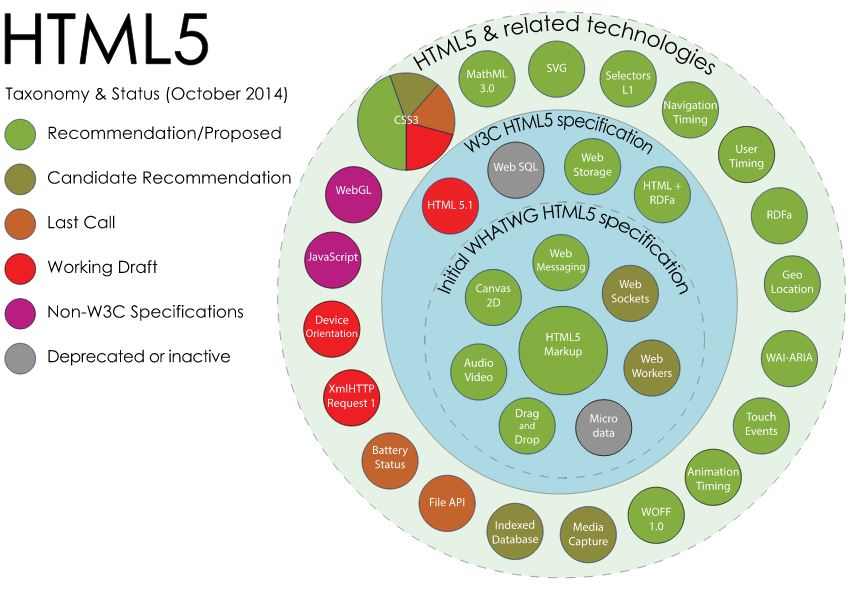
\includegraphics[width=0.7\linewidth]{obrazky/obrazokHTML}
\caption{HTML 5 API}
\label{fig:obrazokHTML}
\end{figure}
\end{center}

HTML5 grafika definuje  dva spôsoby vykreslenia využívajúc: 
\begin{itemize}
	\item $<$canvas$>$ - JavaScript
	\item $<$svg$>$ - SVG
\end{itemize}


\section{Čo je SVG?}
\ac{SVG} je štandardný formát pre vektorovú grafiku. Vektorová grafika je definovaná cez body, priamky, mnohouholníky, elipsy, krivky alebo iné geometrické tvary.  

\acs{SVG} je jazyk na opísanie dvojrozmernej grafiky v   \ac*{XML}. Vďaka tomu, umožňuje reprezentáciu grafických informácii v kompaktnom a prenositeľnom tvare.

 SVG povoľuje tieto tri typy grafických objektov: vektorové grafické tvary, obrázky a text. 
Grafické objekty môžu byť zoskupené, štylizované, zmenené a kombinované do predošlých vrstiev objektov. 

SVG obrázky môžu byť dynamické a interaktívne.

Prispôsobiteľnosť SVG umožňuje zmeniť veľkosť grafického komponentu bez straty kvality vzhľadu, čo umožňuje zobraziť responzívne na viacerých možných zariadení. SVG sa bude zobrazovať rovnako na rôznych platformách. Je kompatibilná s štandardmi \acs{HTML}5, ktoré navrhla \ac*{W3C}. 


 \subsection{Podpora vo webovom prehliadači}
 Súčasné prehliadače plne podporujú $<$svg$>$ elementy.  
  Čísla v tabuľke \ref{svgpreh} špecifikujú prvé verzie webových prehliadačov, ktoré sú schopné zobraziť $<$svg$>$ element.\cite{w3svg}
  
\begin{table}[H]
\begin{center}
		\begin{tabular}{|c|c|c|c|c|c|}
		\hline \textbf{Element} & \textbf{Chrome} & \textbf{Internet} \textbf{Explorer}  & \textbf{Firefox}  & \textbf{Safari} & \textbf{Opera}  \\ 
		\hline $<svg>$ & 4.0& 9.0 & 3.0 & 3.2  &   10.1 \\ 
		\hline 
	\end{tabular} 
\end{center}
	
	\caption{Podpora HTML $<svg>$ elementu v webových prehliadačoch}
	\label{svgpreh}
\end{table}
 
 \begin{figure}[H]
\centering
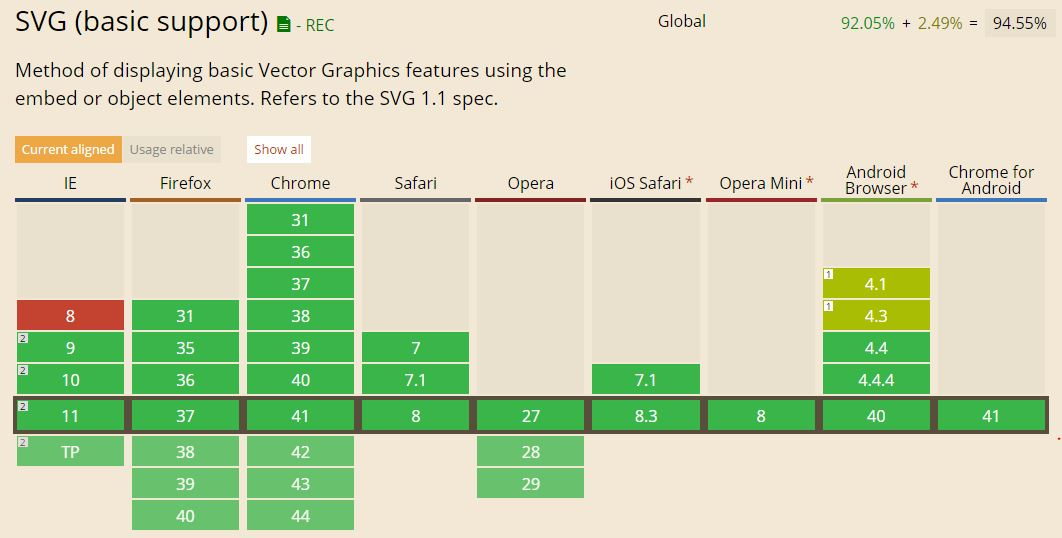
\includegraphics[width=0.7\linewidth]{obrazky/podpora}
\caption{Podpora SVG vo webových prehliadačoch\cite{caniuse2}}
\label{fig:podpora}
\end{figure}

 
 \subsection{Rozdiely medzi SVG a Canvas}

SVG patrí do vektorovej grafiky a Canvas zase do raster bitmap grafiky. SVG je jazyk na opísanie dvojrozmernej grafiky v XML. Canvas kreslí dvojrozmernú grafiku za behu programu cez JavaScript.  SVG je XML založený, čo znamená, že každý element je dostupný cez SVG DOM.  JavaScript umožňuje ovládanie udalostí elementov. V SVG je každý tvar zapamätaný ako objekt.  V prípade zmeny $<$svg$>$ elementu sa automaticky prekreslí.  
 
Canvas je prekresľovaný pixel za pixlom. Bit-mapová grafika je zložitejšia pre dynamické prekresľovanie a má menšie pamäťové nároky a je rýchlejšia. 
 
Zariadenia ako moderné smartfóny majú veľmi vysokú hustotu pixelov. Niektoré potláčajú 300 \ac{PPI} s tým, že sa spoliehajú na obmedzenosť ľudských očí rozoznávať jemné detaily. Pixel nemá v reálnom živote equivalent vo veľkosti, až pokým je na obrazovke s fixovaným rozmerom a rozlíšením. Text s veľkosťou 16 pixlov bude veľmi malý pre oko. Pre tento dôvod zariadenia jednoducho nezobrazujú 1 CSS pixlovú jednotku na 1 pixel zariadenia. Namiesto toho zdvoja svoju veľkosť. \cite{zdrojCSS}

Tabuľka \ref{canvas:SVG} zobrazuje niekoľko dôležitých odlišností medzi Canvas a SVG.\cite{microsoft}%cite 

 \begin{table}[H]
 \centering
	 \begin{tabular}{|p{7.4cm}|p{7.4cm} |}
		\hline \textbf{Canvas} & \textbf{SVG} \\
		\hline Závislé na rozlíšení a \acs{DPI} & Nezávislé na rozlíšení a DPI \\ 
		\hline  Založený na pixloch & Založené na tvaroch \\ 
		\hline Vhodné pre komplexné scény, real-time matematické animácie & Vhodné pre statické obrázky.\\
		\hline Nepodporuje dynamické zmeny & Podporuje dynamické zmeny \\
		\hline Jednoduchý HTML element & Zložený z grafických elementov, ktoré sa stanú časťou DOM \\
		\hline Modifikovateľný len cez script & Modifikovateľné cez script a CSS \\
		\hline Výkonnosť je lepšia s menšou plochou, a väčším množstvom objektov ($>$10 tisíc) &  Výkonnosť je lepšia s menším množstvom objektov ($<$10 tisíc) a väčšou plochou\\ 
		\hline
	 \end{tabular} 
 \caption{Porovnanie Canvas a SVG}
 \label{canvas:SVG}
\end{table}
 
\section{Nástroje na tvorbu grafických komponentov}

\acs{WYSIWYG} editory, ktoré umožňujú tvorbu grafických komponentov sú: 

\begin{itemize}
	\item Inkscape,
	\item CorelDraw, 
	\item  Adobe Illustrator, 
	\item Sketch, 
	\item Libre Office Draw .
\end{itemize}

Voľne dostupné \acs{WYSIWYG} online SVG editory: 
\begin{itemize}
	
	\item svg-edit - Rýchly, webový SVG editor založený na JavaScriptovej technológii, ktorá funguje v akékoľvek modernom webovom prehliadači. \cite{svg-edit}
    \item animatron - online editor, umožnuje vytvoriť HTML5 animácie, a následne exportovať do SVG \acs{SMIL} animácie.\cite{animatron}
	
\end{itemize}

\section{JavaScriptové knižnice pre grafické komponenty}
Na internete sa nachádzajú tieto OpenSource JavaScriptové knižnice na tvorbu grafických komponentov: 
\begin{itemize}
	\item \acs{D3}.js, 
	\item Raphael.js, \item Snap.svg.js,  
	\item Svg.js, 
    \item jQuery.js, \item Velocity.js.
\end{itemize}

Popis jednotlivých JavaScriptových knižníc.
\subsection{D3.js}
D3.js je JavaScriptová knižnica určená na manipuláciu dokumentov založených na dátach. Pomocou \acs{HTML}, \acs{SVG} a \acs{CSS} umožňuje vizualizáciu dát. Je vhodná na vytváranie interaktívnych SVG grafov s hladkými prechodmi a interakciami.  D3 rieši efektívnu manipuláciu dokumentov zakladajúcich si na dátach. Využíva webové štandardy ako \acs{HTML}, \acs{SVG} a \acs{CSS}3. \cite{d3js} Má licenciu BSD.

\subsection{jQuery.js}
JQUery je knižnica s otvoreným zdrojovým kódom, ktorá poskytuje funkcionální programovacie rozhranie k JavaScriptu. Jedná sa o kompletnú knižnicu, ktorej jadro je postavené pomocou selektorov jazyka \acs{CSS} pracujúcimi s elementami modelu \acs{DOM}. Knižnicu jQuery napísal a spravuje John Resig. Má licenciu MIT alebo GPL.  \cite{Zakas}  
V jQuery API metóda animate() umožňuje vytvoriť efekt animácie, ktoré ovplyvňujú CSS vlastnosti. Požadovaný parameter je objekt s CSS vlastnosťami. \cite{jquery}

\subsection{Veloncity.js}
Velocity je nástroj na animáciu s rovnakým \acs{API} ako jQuery  \$.animate(). Funguje aj bez jQuery. Je rýchly, a podporuje animácie farby, transformácie, opakovania, zjemňovania, SVG podpora a rolovanie. \cite{velocity}
Má licenciu MIT. 

\subsection{SVG.js}

SVG.JS je ďalšia knižnica umožňujúca manipulovať a animovať SVG. Medzi hlavné výhody knižnice patrí to, že má ľahko čitateľnú syntax. Umožňuje animovanie veľkosti, pozície, transformácie, farby. Má modulárnu štruktúru, čo umožňuje používanie rôznych rozšírení. Existuje množstvo užitočných pluginov dostupných na internete. \cite{svgjs}
Má licenciu MIT. 

\subsection{Raphaël.js}

Raphaël je malá JavaScriptová knižnica, ktorá umožňuje jednoducho pracovať s vektorovou grafikou na webe. Pomocou jednoduchých príkazov vytvára špecifické grafy, obrázky.  Raphaël využíva \acs{SVG} \acs{W3C} odporúčania a \acs{VML} na tvorbu grafických komponentov. Z toho vyplýva to, že každý vytvorený grafický objekt je zároveň aj DOM objekt. To umožňuje cez JavaScript pridávať manipuláciu udalostí alebo ich upravovať neskôr. Momentálne podporuje Firefox 3.0+, Safari 3.0+, Chrome 5.0+, Opera 9.5+ and Internet Explorer 6.0+.\cite{Raphael}
Autor knižnice je Dmitry Baranovskiy. Raphael \acs{API} má široké spektrum používateľov. Knižnica neumožňuje načítanie SVG do dokumentu zo súboru cez JavaScript. Má licenciu MIT. 

\subsection{Snap.svg.js}

Snap.svg je JavaScriptová knižnica na prácu s SVG. Poskytuje pre webových developerov \acs{API}, ktoré umožňuje animáciu a manipulovanie s buď existujúcim SVG alebo programátorsky vytvorene cez Snap.svg API. Tvorca Snap.svg knižnice je rovnaký ako pri Raphael knižnici.  Bola navrhnutá špeciálne pre moderné prehliadače (IE9 a vyššie, Safari, Chrome, Firefox a Opera). Umožňuje podporu maskovania, strihania, vzorov, plných gradientov, skupín čo doposiaľ nebolo možné pri knižnici Raphael. 

Snap.svg API je schopné pracovať s existujúcim SVG súborom. To znamená, že SVG obsah sa nemusí  generovať cez Snapl.svg API, aby sa mohol oddelene používať. Obrázok vytvorený v nástroji  Inkscape sa dá animovať alebo inak manipulovať cez Snap.svg API. Súbory načítané cez Ajax sa dajú vykresliť, bez toho, aby boli renderované. 

Knižnica Snap.svg podporuje animácie. Poskytuje jednoduché a intuitívne JavaScript API pre vizualizáciu grafických komponentov. Snap.svg umožňuje urobiť SVG obsah viac interaktívnejší a záživnejší. \cite{snapsvg}

\section{Zhodnotenie požiadaviek}

Animovanie cez SVG \acs{SMIL} poskytuje  časovo orientované animácie, ktoré sa spúšťajú v špecifickom intervale a dĺžky. Môžu byť  zobrazované opakovaných sekvenciách. SCADA aplikácie požadujú okamžitú animáciu na zmenu v okamihu, keď  asociované dáta sú aktualizované. Z~toho~robí samotné použitie SVG~SMIL animácií nehodiace sa pre vizualizáciu SCADA systémov. Ďalšia nevýhoda SVG SMIL je, že Internet Expolorer ju nepodporuje.

Použitím JavaScriptových knižníc zameraných na animovanie a manipulovanie s SVG súbormi odstráni problém s SVG SMIL animovaním. Umožnujú používať podmienky, stavy a premenné.

Každá zmena objektu v SCADA systéme sa vykreslí v animácii okamžite bez toho, aby webový prehliadač znovu načítal celú schému. 

Grafické komponenty sa budú vytvárať v programe Inkscape. Následne budú použité v HTML dokumente. Ovládanie a animovanie bude realizované prostredníctvom knižnice Snap.svg. 

Zo spomínaných knižníc najviac vyhovuje práve Snap.svg.js pre splnenie cieľov práce. Ďalší dôvod, prečo som sa rozhodla pre túto  knižnicu bol, že dokáže načítavať SVG súbor a~následné s ním manipulovať. Spĺňa požiadavku kompatibility pre moderné webové prehliadače. Je to open-source knižnica a má licenciu Apache 2.